\documentclass[letterpaper, 14pt, titlepage]{article}

\usepackage{graphicx,amsmath}
\usepackage{fancyvrb}

\usepackage[colorlinks=true, allcolors=blue]{hyperref}

\usepackage{anysize}
\marginsize{1cm}{1cm}{1cm}{1cm}

\usepackage{setspace}
	\onehalfspacing

\usepackage{pdflscape}

\usepackage{tikz, tabularx}
\usetikzlibrary{arrows, fit,positioning}

\author{\Huge George Vega Yon\thanks{\Large gvega at spensiones.cl. Thanks to Damian C. Clarke, F\'elix Villatoro and Eduardo Fajnzylber and the Research team of the Chilean Pension Supervisor for their valuable contributions. The usual disclaimers applies.}\\\\\huge Superintendencia de Pensiones \hspace{1cm} Universidad Adolfo Ib\'a\~nez}

\title{\Huge Introducing PARALLEL: Stata Module for Parallel Computing}

\date{\Large This version \today}

\begin{document}

\begin{landscape}
\maketitle

\clearpage
\LARGE
\section{\Huge Motive}

\begin{itemize}
\item Currently home computers are arriving with extremely high computational capabilities. 
\item Motivated by the video games industry, manufacturers have forged a market for low-cost processing units with the number-crunching horsepower comparable to that of a small supercomputer.

\item In the same way, data availability has improved in a significant manner.
\item Big-Data is an active topic by computer scientists and policy-makers
\item Despite of being available (administrative data) to researchers and policy makers, it has not been exploited as it should.
\item The limited use of these social data resources is not a coincidence. issues involving
\begin{itemize}
\item privacy standardized management
\item lack of statistical computing tools
\end{itemize},  and  are still unsolved both for social scientists, and policy-makers. 
\item {\tt parallel} aims to make a contribution to these issues.
\end{itemize}

\clearpage

\Large
\section{\Huge PARALLEL: Stata module for parallel computing}

Inspired by the R library ``snow'' and to be used in multicore CPUs, {\tt parallel} implements parallel computing methods through OS's shell scripting (using Stata in batch mode) to speedup computations by splitting the dataset into a determined number of clusters\footnote{\normalsize It is important to distinguish between two different ways to understand a cluster. In computer science a \emph{cluster}, or \emph{computer cluster}, refers to a set of computers connected so that they to work as a single system. Here, in the other hand, as this module is intended to be use by statisticians and social scientist in general, I refer to a cluster as a package of data which in this case does not necessary contains related observations (clustered).} in such a way to implement a data parallelism algorithm.

As exposed in \autoref{fig:howitworks}, right after {\tt parallel} splits the dataset into $n$ clusters it starts $n$ new independent stata instances in batch mode over which the same task is simultaneously executed. By default all the loaded instance globals and, optionally, programs and mata objects/programs are passed through. After every cluster stops the resulting datasets are appended and returned to the current stata instance without modifying other elements.

The number of efficient computing clusters depends upon the number of physical cores (CPUs) with which your computer is built, e.g. if you have a quad-core computer, the correct cluster setting should be four. In the case of simultaneous multithreading, such as that from Intel's hyper-threading technology (HTT), setting {\tt parallel} following the number of processors threads, as it was expected, hardly results into a perfect speedup scaling. In spite of it, after several tests on HTT capable architectures, the results of implementing {\tt parallel} according to the machines physical cores versus its logicals shows small though significant differences.

{\tt parallel} is especially handy when it comes to implementing loop-based simulation models (or simply loops), Stata commands such as reshape, or any job that (1) can be repeated through data-blocks, and (2) routines that processes big datasets.

In the case of (pseudo) random number generation, {\tt parallel} allows to set one seed per cluster with the option {\tt seeds(\it{numlist})}.

At this time {\tt parallel} has been successfully tested in Windows and Unix machines. Tests using Mac OS are still pending.

\clearpage

\begin{figure}[tp]
\centering
\caption{\Large How {\tt parallel} works\label{fig:howitworks}}
\bigskip
\scalebox{1.4}{

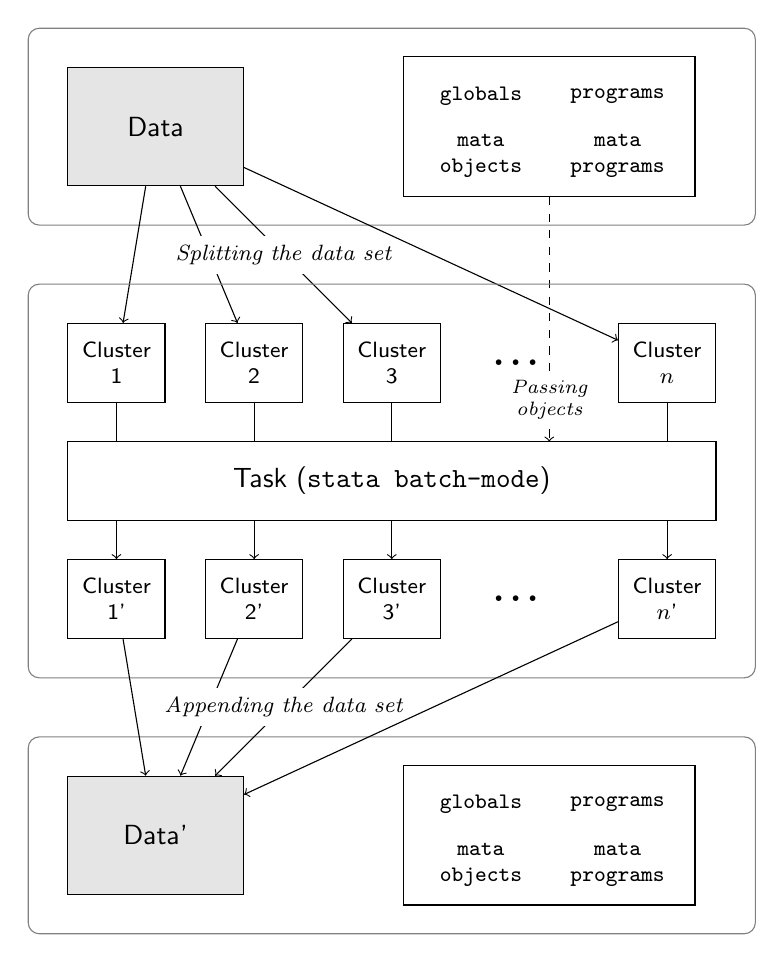
\begin{tikzpicture}[
	every node/.style={node distance=.5cm and .5cm, font=\sffamily}, 
	datablock/.style={rectangle, draw, fill=black!10, text width=2cm, minimum height=1.5cm, text badly centered},
	cluster/.style={rectangle, draw,text width=1cm, text badly centered, minimum height=1cm, font=\footnotesize\sffamily},
	explain/.style={rectangle, text width=5.5cm, align=left, font=\footnotesize\sffamily, node distance=.3, scale=.9}
	] 
	
\node [rectangle, draw=gray, text width=9cm, minimum height=2.5cm, rounded corners] (stata instance0) at (0,0) {};

% Original data
\node [datablock] (data) at (-3,0) {Data};
\matrix [
	draw=black,
	nodes={
		rectangle, text width=1.5cm, minimum height=.75cm, 
		scale=1,
		font=\tt\footnotesize, text badly centered}, column sep=0, row sep=0
	] (others) at (2,0) {
	\node {globals};& \node {programs}; \\
	\node {mata objects}; & \node {mata programs}; \\
};

% Data clusters
\node [cluster] (cluster3) at (0,-3) {Cluster 3};
\node [cluster, left=of cluster3] (cluster2) {Cluster 2};
\node [cluster, left=of cluster2] (cluster1) {Cluster 1};
\node [rectangle, right=of cluster3, text width=1cm, font=\Huge] (threepoints) {...};
\node [cluster, right=of threepoints,text badly centered] (clustern) {Cluster $n$};

% Splitting
\draw[->] (data) -- (cluster1);
\draw[->] (data) -- (cluster2);
\draw[->] (data) -- node [fill=white, font=\footnotesize\it] {Splitting the data set} (cluster3);
\draw[->] (data) -- (clustern);

\draw[->, dashed] (others) -- node [fill=white, font=\scriptsize\it, below=.65cm, text width=1.2cm, minimum height=.7cm,text badly centered] {Passing objects} (2,-4);

% Procesed clusters
\node [cluster] (cluster3p) at (0,-6) {Cluster 3'};
\node [cluster, left=of cluster3p] (cluster2p) {Cluster 2'};
\node [cluster, left=of cluster2p] (cluster1p) {Cluster 1'};
\node [rectangle, right=of cluster3p, text width=1cm, font=\Huge] (threepointsp) {...};
\node [cluster, right=of threepointsp,text badly centered] (clusternp) {Cluster $n$'};

\draw[->] (cluster1) -- (cluster1p);
\draw[->] (cluster2) -- (cluster2p);
\draw[->] (cluster3) -- (cluster3p);
\draw[->] (clustern) -- (clusternp);

% Task
\node [rectangle, draw=gray, text width=9cm, minimum height=5cm, rounded corners] (stata batch) at (0,-4.5) {};
\node [rectangle, fill=white, draw, text width=8cm, text badly centered,minimum height=1cm] (task) at (0,-4.5) {Task (\texttt{stata batch-mode})};

% Result
\node [rectangle, draw=gray, text width=9cm, minimum height=2.5cm, rounded corners] (stata instance1) at (0,-9) {};
\node [datablock] (datap) at (-3,-9) {Data'};
\matrix [
	draw=black,
	nodes={
		rectangle, text width=1.5cm, minimum height=.75cm, 
		scale=1,
		font=\tt\footnotesize, text badly centered}, column sep=0, row sep=0
	] (othersp) at (2,-9) {
	\node {globals};& \node {programs}; \\
	\node {mata objects}; & \node {mata programs}; \\
};

\draw[->] (cluster1p) -- (datap);
\draw[->] (cluster2p) -- (datap);
\draw[->] (cluster3p) -- node [fill=white, font=\footnotesize\it] {Appending the data set} (datap);
\draw[->] (clusternp) -- (datap);

% Text
%\node [explain, right=of stata instance0] {Starting (current) {\tt stata} instance loaded with data plus user defined {\tt globals}, {\tt programs}, {\tt mata objects} and {\tt mata programs}};

%\node [explain, right=of stata batch] {A new {\tt stata} instance (batch-mode) for every data-clusters. Programs, globals and mata objects/programs are passed to them.\\\bigskip The same algorithm (task) is simultaneously applied over the data-clusters.\\\bigskip After every instance stops, the data-clusters are appended into one.};

%\node [explain, right=of stata instance1] {Ending (resulting) {\tt stata} instance loaded with the new data.\\\bigskip User defined {\tt globals}, {\tt programs}, {\tt mata objects} and {\tt mata programs} remind unchanged.};

\end{tikzpicture}

}
\end{figure}

\clearpage
\def\win1{Intel Core i5 M560 (dual-core)}
\def\unix1{Intel Xeon X470 (octa-core)}

\pagebreak

\section{\Huge Example Stata Sesions}

\subsection{\LARGE Reshape (prefix form)}
\begin{Verbatim}[tabsize=4, fontsize=\large]
// Serial fashion
reshape wide tipsolic rutemp opta derecho ngiros, i(numcue) j(tiempo)

// Parallel fashion
parallel, by(numcue) keepl force:reshape wide tipsolic rutemp opta derecho ngiros, ///
	 i(numcue) j(tiempo)
\end{Verbatim}

\subsection{\LARGE Do}
\begin{Verbatim}[tabsize=4, fontsize=\large]
// Serial fashion
parallel "myloop.do"

// Parallel fashion
parallel do "myloop.do"
\end{Verbatim}

\noindent where ``myloop.do'' is
\begin{Verbatim}[tabsize=4, fontsize=\large]
--------------- begin of do-file -------------
local size = _N
forval i=1/`size' {
	qui replace x = 1/sqrt(2*`c(pi)')*exp(-(x^2/2)) in `i'
}
--------------- end of do-file ---------------
\end{Verbatim}

\pagebreak
\section{\Huge Serial replacing using a loop}

\begin{table}[!h]
\Large
\centering
\caption{\large Serial replacing using a loop on a Windows Machine (2 clusters)}
\begin{tabular}{l*{4}{c}}\hline
& \multicolumn{4}{c}{Problem Size} \\
& 10.000 &           100.000 &          1.000.000 &         10.000.000 \\ \hline
CPU &     0.12 &      1.22 &     11.72 &     58.03 \\
Total &     0.81 &      1.53 &      7.96 &     36.13 \\
\hspace{2mm} Setup &     0.02 &      0.08 &      0.56 &      2.86 \\
\hspace{2mm} Compute &     0.55 &      1.20 &      7.10 &     32.65 \\
\hspace{2mm} Finish &     0.25 &      0.25 &      0.30 &      0.62 \\
\hline Ratio (compute) &     0.23 &      1.01 &      1.65 &      1.78 \\
Ratio (total) &     0.15 &      0.80 &      1.47 &      1.61 \\
\hline
\multicolumn{4}{l}{\footnotesize Tested on an \win1 machine}
\end{tabular}
\end{table}

\begin{table}[!h]
\Large
\centering
\caption{\large Serial replacing using a loop on a Linux Server (4 clusters)\label{tab:serialreplace_linux}}
\begin{tabular}{l*{4}{c}}\hline
& \multicolumn{4}{c}{Problem Size} \\
& 10.000 &           100.000 &          1.000.000 &         10.000.000 \\ \hline
CPU &     0.25 &      1.79 &     17.64 &    176.16 \\
Total &     0.45 &      1.00 &      5.14 &     42.61 \\
\hspace{2mm} Setup &     0.02 &      0.11 &      0.81 &      5.16 \\
\hspace{2mm} Compute &     0.23 &      0.67 &      3.86 &     35.98 \\
\hspace{2mm} Finish &     0.21 &      0.23 &      0.46 &      1.47 \\
\hline Ratio (compute) &     1.13 &      2.68 &      4.57 &      4.90 \\
Ratio (total) &     0.56 &      1.79 &      3.43 &      4.13 \\
\hline
\multicolumn{5}{l}{\footnotesize Tested on an \unix1 machine}
\end{tabular}
\end{table}

\pagebreak

\section{\Huge Reshaping a large database}

\begin{table}[!h]
\Large
\centering
\caption{\large Reshaping wide a large database on a Windows Machine (4 clusters with HTT)}
\begin{tabular}{l*{3}{c}}\hline
& \multicolumn{3}{c}{Problem Size} \\
& 100000 &         1000000 &         2000000 \\ \hline
CPU &     4.91 &     50.48 &    106.03 \\
Total &     4.42 &     29.00 &     69.69 \\
\hspace{2mm} Setup &     0.45 &      2.06 &      3.51 \\
\hspace{2mm} Compute &     3.84 &     23.57 &     55.86 \\
\hspace{2mm} Finish &     0.13 &      3.37 &     10.31 \\
\hline Ratio (compute) &     1.28 &      2.14 &      1.90 \\
Ratio (total) &     1.11 &      1.74 &      1.52 \\
\hline
\multicolumn{4}{l}{\footnotesize Tested on an \win1 machine}
\end{tabular}
\end{table}

\begin{table}[!h]
\Large
\centering
\caption{\large Reshaping wide a large database on a Linux Server (4 clusters)}
\begin{tabular}{l*{3}{c}}\hline
& \multicolumn{3}{c}{Problem Size} \\
& 100.000 &          1.000.000 &         5.000.000 \\ \hline
CPU &     9.00 &    101.94 &    564.13 \\
Total &     4.41 &     43.92 &    317.60 \\
\hspace{2mm} Setup &     0.77 &      1.43 &     10.03 \\
\hspace{2mm} Compute &     3.17 &     38.52 &    283.05 \\
\hspace{2mm} Finish &     0.47 &      3.98 &     24.53 \\
\hline Ratio (compute) &     2.84 &      2.65 &      1.99 \\
Ratio (total) &     2.04 &      2.32 &      1.78 \\
\hline
\multicolumn{4}{l}{\footnotesize Tested on an \unix1 machine}
\end{tabular}
\end{table}

\pagebreak

\section{\Huge Monte Carlo Simulation}

\begin{table}[!h]
\Large
\centering
\caption{\large Monte Carlo Experiment on a Windows Machine}
\begin{tabular}{l*{2}{c}}\hline
& \multicolumn{2}{c}{Number of Clusters} \\
& 2 &               4 \\ \hline
CPU &    28.50 &     28.92 \\
Total &    17.49 &     18.30 \\
\hspace{2mm} Setup &     0.11 &      0.12 \\
\hspace{2mm} Compute &    17.27 &     18.07 \\
\hspace{2mm} Finish &     0.11 &      0.11 \\
\hline Ratio (compute) &     1.65 &      1.60 \\
Ratio (total) &     1.63 &      1.58 \\
\hline
\multicolumn{3}{c}{\footnotesize Tested on a \win1 machine}
\end{tabular}
\end{table}

\begin{table}[!h]
\Large
\centering
\caption{\large Monte Carlo Experiment on a Linux Server}
\begin{tabular}{l*{3}{c}}\hline
& \multicolumn{3}{c}{Number of Clusters} \\
& 2 &               3 &               5 \\ \hline
CPU &    40.97 &     39.01 &     36.44 \\
Total &    18.35 &     15.20 &      7.62 \\
\hspace{2mm} Setup &     0.11 &      0.11 &      0.12 \\
\hspace{2mm} Compute &    18.13 &     14.99 &      7.41 \\
\hspace{2mm} Finish &     0.10 &      0.10 &      0.10 \\
\hline Ratio (compute) &     2.26 &      2.60 &      4.92 \\
Ratio (total) &     2.23 &      2.57 &      4.78 \\
\hline
\multicolumn{4}{c}{\footnotesize Tested on a \unix1 machine}
\end{tabular}
\end{table}

\pagebreak


\end{landscape}

\end{document}